\renewcommand{\thispart}{1 }
\renewcommand{\thispartname}{Introduction to Machine Learning}

\part{\thispartname}

% Cover page
%
% Cover page for giveb part
%

\title[\modulename - Part \thispart]
{
  {\bf 
   \modulename - 
   Part \thispart\\
  }
  \vspace{0.5cm}
  {\it 
   \color{yellow}
    \secname\\
  }
}
\author[C.Andreopoulos] {
  Professor Costas Andreopoulos\inst{1,2}, {\it FHEA}
}
\institute[Liverpool/STFC-RAL] {
   \inst{1} University of Liverpool, Department of Physics\\
   \vspace{0.3cm}
   {\it {\color{magenta} Lectures delivered at the University of Liverpool, 2024-25}}\\
   \vspace{0.2cm}
}
\date{\today}

\titlegraphic{
  
\includegraphics[height=30px]{images/logo/liverpool.png}
}

\begin{frame}[plain]
  \titlepage
\end{frame}




% Outline
\section{Outline}
%
% Table of contents to be displayed at the beginning of each part
%

\begin{frame}[t,allowframebreaks]{Outline for Part \thispart -}
  % Part \thispart (\secname) covers the following topics:\\
  % \vspace{0.5cm}
  \linespread{1.1}
  \setcounter{secnumdepth}{3}
  \setcounter{tocdepth}{3}
  % \tableofcontents[currentsection, hideothersubsections, sectionstyle=hide/hide]
  \tableofcontents[part=\thispart]
\end{frame}



% AI
\section{Artificial intelligence}
\begin{frame}{Artificial Intelligence}

    \index{artificial intelligence}\index{AI}\gls{ai} 
    can be defined as the 
    `{\bf science and engineering of making intelligent 
    machines}' \cite{McCarthy:2007ai}.\\
    \vspace{0.2cm}
    Intelligence: 
    \begin{itemize}
        \item can be difficult to define \cite{Neisser:1996intl},
        \item is an umbrella term for several skills and abilities, and
        \item is generally understood in relation to human intelligence \cite{McCarthy:2007ai}.\\
    \end{itemize}
    \vspace{0.1cm}
    \begin{block}{}
    Generally, intelligence is the capacity to {\bf acquire information}, 
    {\bf convert it to knowledge}, and {\bf apply that knowledge} 
    to think abstractly or while interacting with the environment.\\
    \end{block}
    \vspace{0.1cm}
    There are many types of intelligence.\\
    \vspace{0.1cm}
    Humans, animals, and some machines display varying levels of intelligence.\\
    
\end{frame}
    

% Precursors of AI
\section{Precursors of artificial intelligence}
%
%
%

\begin{frame}[t, allowframebreaks]{Precursors of Artifial Intelligence -}

    \vspace{-0.1cm}
    We always dreamt of {\bf building machines with human-like intelligence}!\\
    \begin{itemize}
        \small
        \item
        Master craftsmen and intelligent machines in many myths and stories.\\
    \end{itemize}
    \vspace{-0.4cm}

    \begin{columns}[t]
        \begin{column}{0.46\textwidth}
         \begin{center}
          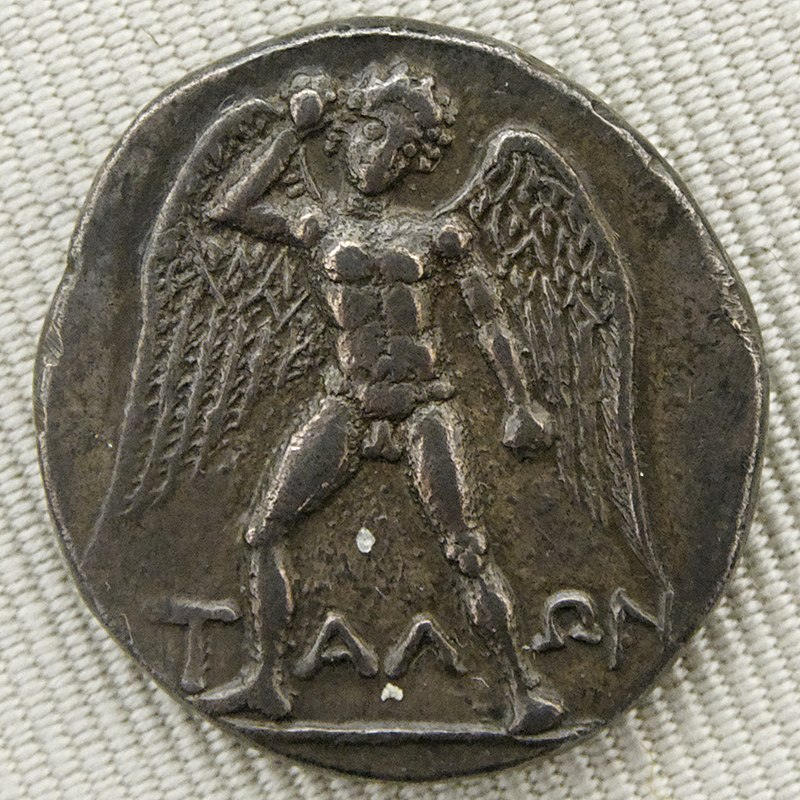
\includegraphics[width=0.99\textwidth]{./images/precursors/talos.jpg}\\
          {\scriptsize 
          \vspace{0.1cm}
          Talos on a Greek coin from 300 BCE.\\
          \color{col:attribution} 
          (Cabinet des Médailles, Paris.)
          \href{https://en.wikipedia.org/wiki/Talos\#/media/File:Didrachm_Phaistos_obverse_CdM.jpg}{\tiny [link]}
          \\}
         \end{center}
        \end{column}
        \begin{column}{0.54\textwidth}
            \begin{itemize}
                \small
                \item 
                {\bf Talos}, the bronze giant built by the god
                Hephaestus to protect Crete from invaders.
                \href{https://en.wikipedia.org/wiki/Talos}{\tiny [Wikipedia]}
                \item 
                {\bf Galatea}, the female ivory statue animated 
                by the goddess Aphrodite when its sculptor, Pygmalion, 
                fell in love with it.
                \href{https://en.wikipedia.org/wiki/Pygmalion_(mythology)}{\tiny [Wikipedia]}
                \item
                {\bf Golems} in Jewish folklore, made from clay 
                and animated by words written on their foreheads, 
                or on pieces of paper placed in their mouth.
                \href{https://en.wikipedia.org/wiki/Golem}{\tiny [Wikipedia]}
                \item
                {\bf Homunculi} (sing.: Homunculus), 
                the little anthropomorphic creatures found in alchemical traditions.
                \href{https://en.wikipedia.org/wiki/Homunculus}{\tiny [Wikipedia]}
            \end{itemize}        
        \end{column}
    \end{columns}

    \framebreak

    \begin{itemize}
        \small
        \item
        {\bf Brazen heads}, the future-telling automata of 
        Gerbert of Aurillac, Saint Albertus, Robert Grosseteste, 
        and Roger Bacon.
        \href{https://en.wikipedia.org/wiki/Brazen_head}{\tiny [Wikipedia]}\\
        \item
        {\bf Frankenstein!} by Marry Shelley (1818).
        
\includegraphics[width=0.04\textwidth]{./images/precursors/stein.jpg}
        \href{https://en.wikipedia.org/wiki/Frankenstein}{\tiny [Wikipedia]}\\
        \item
        {\bf Hadaly}, the female android in the science fiction novel `The Future Eve' (1886)
        by Auguste Villiers de I'Isle-Adam.
        \href{https://en.wikipedia.org/wiki/The_Future_Eve}{\tiny [Wikipedia]}\\
        \item
        {\bf Maria} in the science fiction movie `Metropolis' (1927)
        \href{https://en.wikipedia.org/wiki/Metropolis_(1927_film)}{\tiny [Wikipedia]}\\
    \end{itemize}        

    \vspace{-0.3cm}

    \begin{columns}[t]
        \begin{column}{0.32\textwidth}
            \begin{center}
                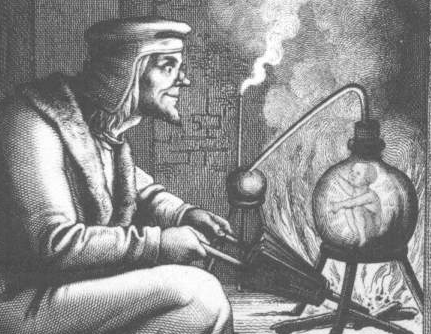
\includegraphics[width=0.99\textwidth]
                {./images/precursors/homunculus_cropped.png}\\
                {\scriptsize 
                \vspace{0.1cm}
                19$^{th}$ century engraving of Wagner and Homunculus 
                from Goethe's Faust II.
                \href{https://en.wikipedia.org/wiki/Homunculus\#/media/File:Faust_image_19thcentury.jpg}{\tiny [link]}\\
                }
            \end{center}
        \end{column}
        \begin{column}{0.37\textwidth}
            \begin{center}
                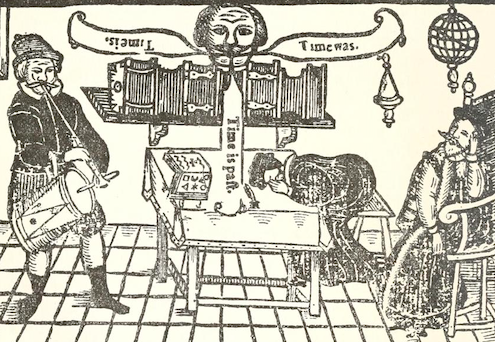
\includegraphics[width=0.99\textwidth]
                {./images/precursors/brazen_head_cropped.png}\\
                {\scriptsize 
                \vspace{0.1cm}
                Reprint of 1630 edition of 
                Robert Greene's Friar Bacon and Friar Bungay.
                \href{https://en.wikipedia.org/wiki/Friar_Bacon_and_Friar_Bungay\#/media/File:Greene_Bacon_and_Bungay_1630.jpg}{\tiny [link]}\\
                }
            \end{center}
        \end{column}
        \begin{column}{0.30\textwidth}
            \begin{center}
                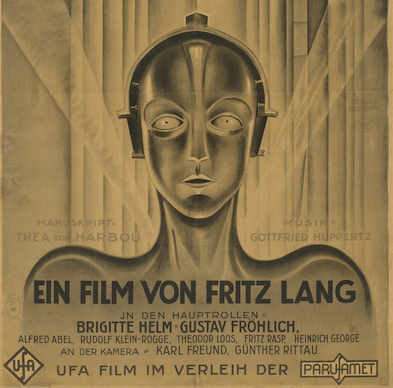
\includegraphics[width=0.80\textwidth]
                {./images/precursors/metropolis_cropped.png}\\
                {\scriptsize 
                \vspace{0.1cm}
                Part of the theatrical release poster for Metropolis,
                by Heinz Schulz-Neudamn.
                \href{https://en.wikipedia.org/wiki/Metropolis_(1927_film)\#/media/File:Metropolis_(German_three-sheet_poster).jpg}{\tiny [link]}\\
                }      
            \end{center}
        \end{column}
    \end{columns}

\end{frame}

% Types of AI
\section{Types of artificial intelligence}

%
%
%

\begin{frame}{Types of Artifical Intelligence}

    Classification based on capabilities (Type-1):\\
    \vspace{0.1cm}

    \begin{itemize}

        \item 
        \index{artificial narrow intelligence}\index{ANI}
        \gls{ani}, often referred to as 
        \index{weak AI}\Gls{weak ai} or
        \index{narrow AI}\Gls{narrow ai}:
        This is \index{artificial intelligence}\index{AI}\gls{ai} 
        with a {\bf narrow range of capabilities}.\\

        \vspace{0.1cm}

        \begin{itemize}
            \item 
            Only type of \gls{ai} that is {\bf successfully implemented to date}
            \item
            Examples: 
            self-driven cars, voice assistants, 
            face recognition tools, spam filters,
            news feed personalization in social media, 
            chatbots etc.
            \item 
            Trained for specific tasks in a {\bf narrow domain}.   
            \item 
            {\bf Imitates intelligence}, rather than being intelligent.\\
        \end{itemize}

        \vspace{0.1cm}

        \item 
        \index{artificial general intelligence}\index{AGI}
        \gls{agi}, often referred to as 
        \index{strong AI}\Gls{strong ai} or
        \index{deep AI}\Gls{deep ai}:
        \gls{ai} with {\bf human-level capabilities}.\\

        \vspace{0.1cm}

        \begin{itemize}
            \item 
            {\bf Autonomous systems} that {\bf can learn any task}.
            \item 
            Currently, there is no such system.
            \item
            72 \index{agi} R\&D projects were identified as being active in 2020 \cite{GCRI:2020agi}.
        \end{itemize}


        \vspace{0.1cm}
        \item 
        \index{artificial superintelligence}\index{ASI} 
        \gls{asi}:
        \gls{ai} that greatly {\bf exceeds human capabilities} - A hypothetical concept.

    \end{itemize}
    
\end{frame}

%

\begin{frame}{Types of Artifical Intelligence}

    Classification based on functionality (Type-2):\\

    \begin{itemize}

        \item 
        \index{reactive AI}\index{artificial intelligence}\index{AI}\Gls{reactive ai}
        \begin{itemize}
            \item 
            Task-specific \gls{ai} that reacts to inputs and is 
            predictable (it always produces a given response for a given set of inputs)
            \item 
            Does not store memories and does not learn from experience.
            \item
            Example: IBM's Deep Blue chess-playing \gls{ai} system
        \end{itemize}

        \item 
        \index{limited memory AI}\Gls{limited memory ai}
        \begin{itemize}
            \item 
            Task-specific \gls{ai} that stores memories (for a limited time period) 
            and learns from its experiences.
            \item
            Example: Self-driven cars
        \end{itemize}

        \item 
        \index{theory of mind AI}\Gls{theory of mind ai}
        \begin{itemize}
            \item 
            Next-level \gls{ai} system, able to learn any task and exhibit common sense.
            \item 
            Emotionally intelligent, would be able to interact with human emotions
            and adjust its behaviour, show empathy, and understand moral norms.
        \end{itemize}

        \item 
        \index{self-awareness AI}\Gls{self-awareness ai}
        \begin{itemize}
            \item Would attribute mental states not only to others, but also to self.
            \item \gls{ai} with human-level artificial consciousness.
        \end{itemize}

    \end{itemize}
    
\end{frame}


%
%
%

\begin{frame}[t]{Intelligence?} 

    Imitating intelligence, let alone achieving genuine 
    intelligence, is very hard!\\
    \vspace{0.2cm}

    \begin{columns}
        \begin{column}{0.27\textwidth}
         {\small
           A small sample of \index{AI}\gls{ai} failures that hit the 
           news recently are listed on the right.\\
         }   
         \begin{center}
          
\includegraphics[width=0.98\textwidth]{./images/misc/malfunctioning_robot_1.png}\\
         \end{center}
        \end{column}
        \begin{column}{0.73\textwidth}        
            \begin{itemize}
                \small
                \item 
                Teslas running Autopilot involved in 273 crashes reported in 2021-22.
                \href{https://www.washingtonpost.com/technology/2022/06/15/tesla-autopilot-crashes/}
                {\small [$\rightarrow$ Washington Post article]}
                \item 
                False facial recognition match leads to Black man’s arrest.                
                \href{https://edition.cnn.com/2021/04/29/tech/nijeer-parks-facial-recognition-police-arrest/index.html}
                {\small [$\rightarrow$ CNN article]}
                \item 
                OpenAI GPT-3 medical chatbot designed to help doctors manage 
                their daily workload, told a mock patient to kill themselves.
                \href{https://www.theregister.com/2020/10/28/gpt3_medical_chatbot_experiment/}
                {\small [$\rightarrow$ The Register article]}
                \item 
                A beauty contest was judged by AI and the robots didn't like dark skin.
                \href{https://www.theguardian.com/technology/2016/sep/08/artificial-intelligence-beauty-contest-doesnt-like-black-people}
                {\small [$\rightarrow$ The Guardian article]}
                \item 
                New Zealand passport robot tells applicant of Asian descent to open eyes.
                \href{https://www.reuters.com/article/us-newzealand-passport-error-idUSKBN13W0RL}
                {\small [$\rightarrow$ Reuters article]}
                \item 
                Tay, Microsoft's pro-nazi anti-feminist AI chatbot.\\
                \href{https://www.theguardian.com/technology/2016/mar/24/tay-microsofts-ai-chatbot-gets-a-crash-course-in-racism-from-twitter}
                {\small [$\rightarrow$ The Guardian article]}
            \end{itemize}

        \end{column}
    \end{columns}

    \vspace{0.2cm}
    {\small
      A large list of hilarious failures, mainly from gaming \gls{ai}, 
      is maintained at \cite{GoogDoc:GamingExamplesinAI}.
    }

\end{frame}

% \begin{itemize}
%     \small
%     \item 
%     Neural nets evolved to classify edible and poisonous 
%     mushrooms took advantage of the data being presented 
%     in alternating order, and didn't actually learn any 
%     features of the input images \cite{Lehman:2019Surprising}
%     \item 
%     PlayFun algorithm deliberately dies in the Bubble Bobble 
%     game as a way to teleport to the respawn location
%     \item 
%     Creatures bred for speed grow really tall and 
%     generate high velocities by falling over
%     \item 
%     In an artificial life simulation where survival required 
%     energy but giving birth had no energy cost, one species 
%     evolved a sedentary lifestyle that consisted mostly of 
%     mating in order to produce new children which could be 
%     eaten (or used as mates to produce more edible children).
%     \item 
%     Agent kills itself at the end of level 1 to avoid losing in level 2
%     \item 
%     In a football game, the player is supposed to try 
%     to score a goal against the goalie, one-on-one. 
%     Instead, the player kicks it out of bounds. 
%     Someone from the other team has to throw the 
%     ball in (in this case the goalie), so now the player has a clear shot at the goal.
%     \item 
%     Rewarding a football robot for touching the ball 
%     caused it to learn to get to the ball and vibrate 
%     touching it as fast as possible
%     \item 
%     CycleGAN algorithm for converting aerial photographs 
%     into street maps and back, trained to minimise the cyclic 
%     consistency loss, encoded output information in the intermediary 
%     image without it being humanly detectable.
% \end{itemize}        



% History of AI
\section{History of artificial intelligence}
\begin{frame}{The history of AI\footnote{
\tiny For a detailed discussion, see \url{https://en.wikipedia.org/wiki/History_of_artificial_intelligence}}}

\begin{itemize}
\item Birth of AI (1952-1956)
\item Symbolic AI (1956-1974)
\item First AI winter (1974-1980)
\item Boom (1980-1987)
\item Bust: Second AI winter (1987-1993)
\item AI (1993-2011)
\item Deep learning, big data and AI (2011-present)

\end{itemize}

\end{frame}


\subsection{Birth of AI (1952-1956)}
%
%
%

\begin{frame}[t]{Birth of AI (1952-1956)} 

    Several developments in the first half of the 20th century:
    \begin{itemize}
        \item Discovery that the {\bf brain is an electrical network of neurons}
        \begin{itemize}
            \item 
              Richard Caton reported to British Medical Association 
              the first observation of electrical impulses from the 
              brains of living animals (1875) \cite{Caton:1875}.
            \item 
              Hans Berger recorded the first human 
              electroencephalogram (1924) \cite{Berger:1929}.
        \end{itemize}
        \item 
        Development of {\bf control and communication theory} (cyberneutics) 
        \begin{itemize}
            \item by Norbert Wiener
        \end{itemize}
        \item 
        Development of {\bf information theory} 
        \href{https://en.wikipedia.org/wiki/Information_theory}{\tiny [Wikipedia]}
        \begin{itemize}
            \item Early work by Harry Nyquist and Ralph Hartley in 1920's.
            \item Foundations established by Claude Shannon in the 1940's \cite{Shannon:1948}.
        \end{itemize}
        \item 
        Development of {\bf theory of computation} 
        \href{https://en.wikipedia.org/wiki/Theory_of_computation}{\tiny [Wikipedia]}
        \begin{itemize}
            \item John von Neumann, Alan Turing, Alonzo Church and others
        \end{itemize}
    \end{itemize}
    \vspace{0.2cm}
    In early 1950's it became possible to {\bf start imagining a digital brain}!
            
\end{frame}
    
    
    
%
%
%

\begin{frame}[t]{Turing's `Computing Machinery and Intelligence' (1950)} 

    Landmark paper by \gls{Turing}\cite{Turing:1950tt} - Possibility of creating machines that think
    Turing test

\end{frame}

\begin{frame}[t]{SNARC (1951)} 

A first neural net machine, \gls{snarc}, 
was built by \gls{Minsky} and \gls{Edmonds} in 1951.

\begin{columns}
    \begin{column}{0.45\textwidth}
      They design of \gls{snarc} drew inspiration from the work of 
      \gls{McCulloch} and \gls{Pitts} on
      artificial neurons.           
     \begin{center}
        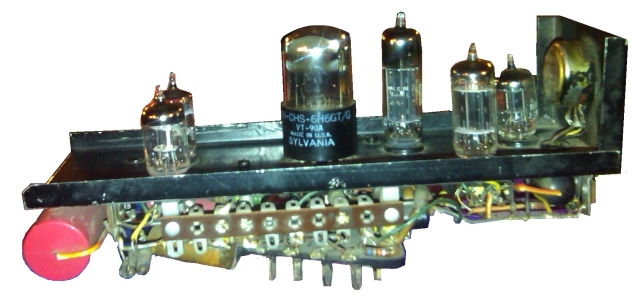
\includegraphics[width=0.99\textwidth]
        {./images/snarc/gregoryloan_snarc_hebbsynapse.png}\\
     {\scriptsize 
      A photograph by Gregory Loan of the only surviving \gls{snarc} neuron.\\
      \color{col:attribution} 
      Photo reproduced from \cite{CyberneticZoo:1951MazeSolver}}\\
     \end{center}
    \end{column}
    \begin{column}{0.55\textwidth}
       \begin{itemize} 
        \item
        \gls{snarc} was a randomly connected network 
        of about 40 neurons (Hebb synapses).
        \item
        Each neuron had a short-term memory and a long-term memory.
        \item
        The machine was trained by navigating a virtual maze 
        (i.e. \gls{snarc} was a "mechanical rat").
        \item
        Actions resulting to a positive reward (provided manually 
        by an operator), engaged a chain that turned a potentiometer 
        (whose setting was analogous to a weight in modern digital networks).
       \end{itemize}
    \end{column}
\end{columns}

\end{frame}
%
%
%

\begin{frame}[t]{Logic Theorist} 

Logic Theorist was a computer program that could perform 
some level of automated reasoning. \cite{Newell:1956logth}
    
\end{frame}
%
%
%

\begin{frame}[t,allowframebreaks]{Dartmouth conference (1956) -} 

    \vspace{-0.2cm}

    \begin{columns}
        \begin{column}{0.62\textwidth}
            \begin{center}
            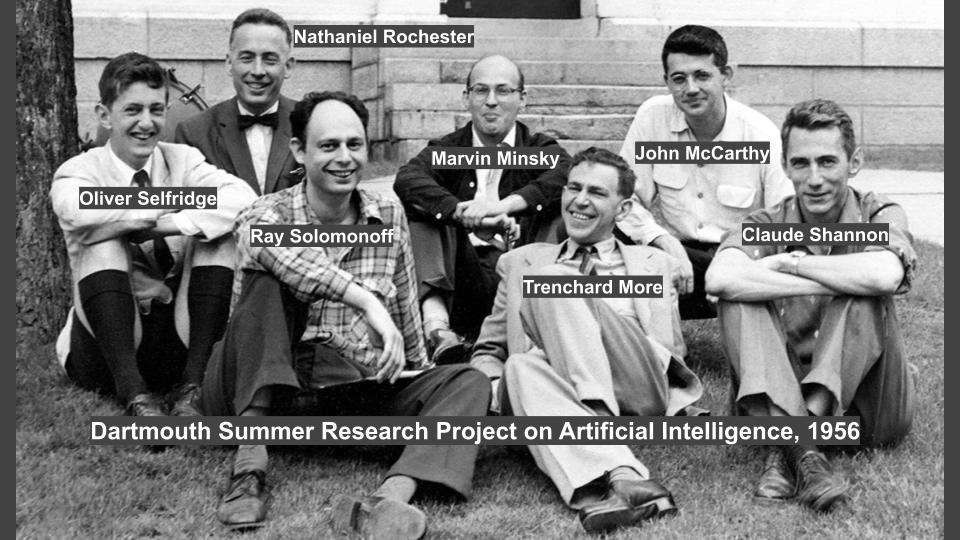
\includegraphics[width=0.98\textwidth]{./images/people/dartmouth_1956.jpg}\\
            { \scriptsize 
            \vspace{0.1cm}
            Participants in the Dartmouth Summer Research Project 
            on Artificial Intelligence, 1956.\\
            \color{col:attribution} 
            Photo labelled by Mindy McAdams
            \href{https://twitter.com/macloo/status/1319683530742431748/photo/1}{\tiny [link]}
            \\}
            \end{center}
        \end{column}
        \begin{column}{0.38\textwidth}
            \begin{blockexample}{} 
            {\tt 
                \scriptsize
                "Every aspect of learning or any other 
                feature of intelligence can in principle 
                be so precisely described that a machine can be made 
                to simulate it. An attempt will be made to find how 
                to make machines use language, form abstractions and 
                concepts, solve kinds of problems now reserved for humans, 
                and improve themselves. We think that a significant advance 
                can be made in one or more of these problems if a carefully 
                selected group of scientists work on it together for a summer."\\
            } 
           \vspace{0.2cm}
            {\scriptsize
                 A Proposal for the Dartmouth Summer Research Project 
                 on Artificial Intelligence \cite{Dartmouth:1956}.\\
            }
            \end{blockexample}
        \end{column}
    \end{columns}

    \framebreak

    \begin{blockexample}{} 
        {\tt 
            \scriptsize
            "Anybody who was there was pretty stubborn about pursuing 
            the ideas that he had before he came, nor was there, 
            as far as I could see, any real exchange of ideas."\\
            %People came for different periods of time. 
            %The idea was that everyone would agree to come for six weeks, 
            %and the people came for periods ranging from two days to 
            %the whole six weeks, so not everybody was there at once. 
            %It was a great disappointment to me because it really meant 
            %that we couldn’t have regular meetings."\\
        } 
       \vspace{0.2cm}
        {\scriptsize
             Someone \cite{Dartmouth:1956}.\\
        }
    \end{blockexample}

    \begin{blockexample}{} 
        {\tt 
            \scriptsize
            "They didn't want to hear from us, and we sure didn't want to hear 
            from them: we had something to show them! ... 
            In a way it was ironic because we already had done the first example 
            of what they were after; and second, they didn't pay much attention to it."\\
        } 
       \vspace{0.2cm}
        {\scriptsize
             H.Simon, co-creator of the Logical Theorist \cite{Crevier:1993}.\\
        }
    \end{blockexample}

    \begin{columns}
        \begin{column}{0.30\textwidth}
            \begin{center}
            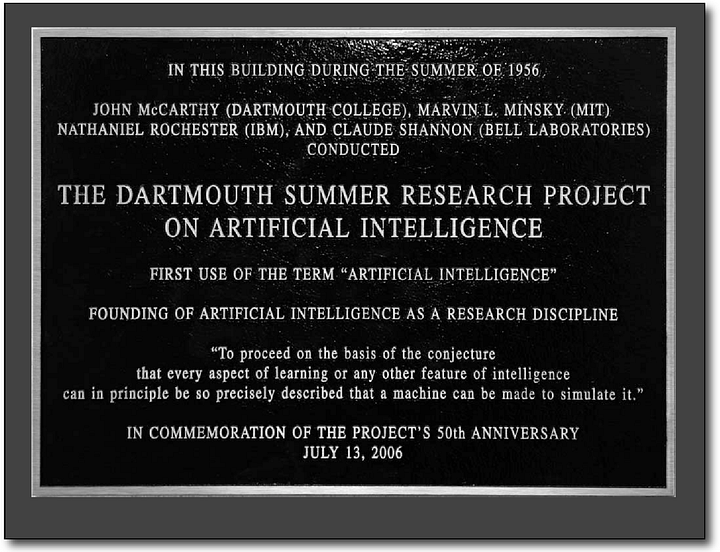
\includegraphics[width=0.98\textwidth]{./images/misc/dartmouth_commemorative_plaque.png}\\
            { \scriptsize 
            \vspace{0.1cm}
            Dartmouth Hall Commemorative Plaque..\\
            \color{col:attribution} 
            Photo by Joe Mehling, taken from \cite{Veisdal:2019dartmouth}.\\}
            \end{center}
        \end{column}
        \begin{column}{0.70\textwidth}
        \end{column}
    \end{columns}

\end{frame}


\subsection{Symbolic AI (1956-1974)}
\subsection{First AI winter (1974-1980)}
\subsection{Boom (1980-1987)}
\subsection{Bust: Second AI winter (1987-1993)}
\subsection{AI (1993-2011)}
\subsection{Deep learning, big data and AI (2011-present)}


%
%
%

\begin{frame}[t]{Effect of increased data}

    \begin{columns}
        \begin{column}{0.50\textwidth}
         \begin{center}
          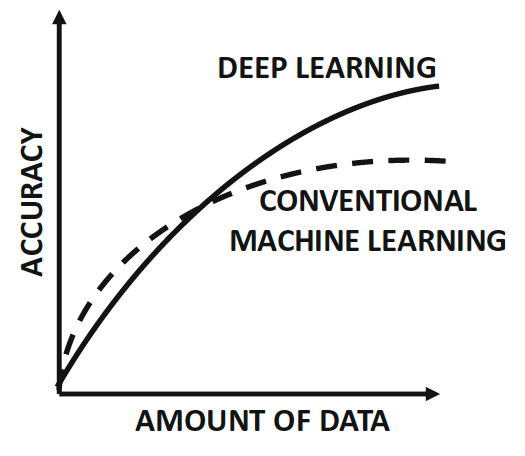
\includegraphics[width=0.95\textwidth]{./images/dl_intro/accuracy_vs_amount_of_data_1.png}\\
          {\scriptsize \color{col:attribution} 
          Image reproduced from p.54 of \cite{Aggarwal:2018SpringerDL}}\\
         \end{center}
        \end{column}
        \begin{column}{0.50\textwidth}
        \end{column}
    \end{columns}


\end{frame}

%
%
%

\begin{frame}[t,allowframebreaks]{Increasing neural network size - }

    % Intro

    % Number of connections in various artificial neural nets as a function of time
    % and comparison with biological brains

    The human brain has $\sim$100 billion neurons and $\sim$100 trillion synapses!

    \begin{center}
        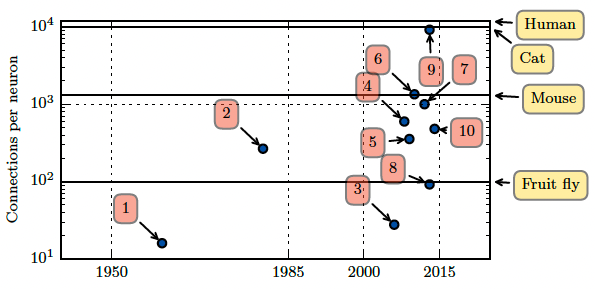
\includegraphics[width=0.95\textwidth]
          {./images/dl_intro/nnet_size_connections_vs_time_01.png}\\
        {\scriptsize \color{col:attribution} 
        Reproduced from p.22 of \cite{Goodfellow:2017DL}}\\
    \end{center}

    \framebreak

    % Number of neurons in various artificial neural nets as a function of time
    % and comparison with biological brains

    \begin{center}
        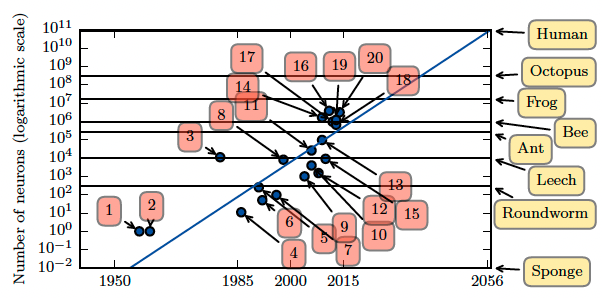
\includegraphics[width=0.95\textwidth]
           {./images/dl_intro/nnet_size_neurons_vs_time_01.png}\\
        {\scriptsize \color{col:attribution} 
        Reproduced from p.23 of \cite{Goodfellow:2017DL}}\\
    \end{center}
       {\tiny
       1. Perceptron (1958) \cite{Rosenblatt:1958p},
       2. Adaptive linear element (1960) \cite{Widrow:1960as},
       3. Neocognitron (1980) \cite{Fukushima:1980nc},
       4. Early back-propagation network (1986) \cite{Rumelhart:1986erp},
       5. Recurrent neural network for speech recognition (1991) \cite{Robinson:1991rerp},
       6. Multilayer perceptron for speech recognition (1991) \cite{Bengio:1991pma},
       7. Mean field sigmoid belief network (1996) \cite{Saul:1996mf},
       8. LeNet-5 (1998) \cite{LeCun:1998ln5},

       9. Echo state network (2004) (Jaeger and Haas, 2004)
       10. Deep belief network (2006) (Hinton et al., 2006)
       11. GPU-accelerated convolutional network (2006) (Chellapilla et al., 2006)
       12. Deep Boltzmann machine (2009) (Salakhutdinov and Hinton, 2009a)
       13. GPU-accelerated deep belief network (2009) (Raina et al., 2009)
       14. Unsupervised convolutional network (2009) (Jarrett et al., 2009)
       15. GPU-accelerated multilayer perceptron (2010) (Ciresan et al., 2010)
       16. OMP-1 network (2011) (Coates and Ng, 2011)
       
       17. Distributed autoencoder (2012) \cite{Le:2012daut}
       18. Multi-GPU convolutional network (2012) \cite{Krizhevsky:2012img},
       19. COTS HPC unsupervised convolutional network (2013) \cite{Coates:2013cots},       
       20. GoogLeNet (2014) \cite{Szegedy:2014gnet}\\
       }

    \framebreak

    % Information from recent well-known artificial neural networks

    \begin{itemize}
        \item GPT-2 had 1.5 billion parameters and around 50 billion neurons
        \item GPT-3 is estimated to have around 60-80 billion neurons
        \item GPT-4 is estimated to have around 60-80 billion neurons
    \end{itemize}

\end{frame}


\section{Human vs computer learning}
%
%
%


\begin{frame}[t,allowframebreaks]{Human vs computer intelligence -} 

\begin{itemize}
\item Computers can 
\end{itemize}

\end{frame}

\section{Different learning paradigms: Supervised, unsupervised and reinforcement learning}

\section{Artificial intelligence, machine learning and deep learning}

\section{Machine learning tasks}

\section{A simple practical example: Linear regression}

\section{Biologically inspired methods of computer learning}

\section{Basic architecture of neural networks}

\section{Fundamental concepts}
\begin{frame}[t,allowframebreaks]{Fundamental concepts - }

    \gls{relu}
\end{frame}


% From AI to DL
\begin{frame}{Connection between AI, ML and DL}

\index{AI}\index{artificial intelligence}\gls{ai} -
\gls{ai}
\gls{ml}
\gls{dl}

    \begin{center}
        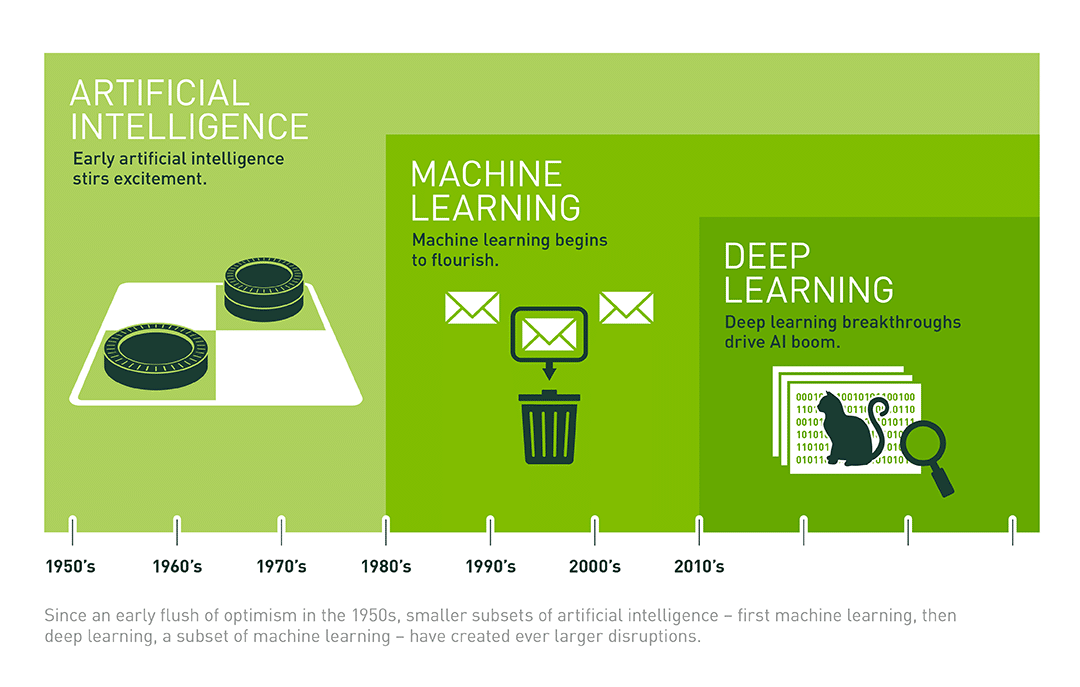
\includegraphics[width=0.90\textwidth]{./images/dl_intro/ai_ml_dl.png}\\
        {\scriptsize Image reproduced from \cite{NVidiaBlog:DifferenceBetweenAIMLDL}}\\
    \end{center}

\end{frame}
    


% Main points to remember
\renewcommand{\summarizedlecture}{1 }

%
%
%

\begin{frame}{Lecture \summarizedlecture - \lecturesummarytitle}


\end{frame}



% Suggested reading for this part
\section{Suggested reading}
%
%
%

\begin{frame}{Suggested reading for Part \thispart}

    {
        \small
        Essential reading on {\bf automatic differentiation}:
        \begin{itemize}
            \scriptsize
            \item Section 6.5 from the `Deep Learning' 
            textbook of Goodfellow, Bengio and Courville \cite{Goodfellow:2017MITDL}.
            \item Appendix B from the `Machine Learning Refined' 
            textbook of Watt, Borhani and Katsaggelos \cite{Watt:2016Cambridge}.
            \item `A review of automatic differentiation and its 
            efficient implementation' by Margossian \cite{Margossian:2019ad}
        \end{itemize}
        
        Also, you may want to browse:
        \begin{itemize}
            \scriptsize
            \item The collection of articles
             in the book `Automatic Differentiation: Applications, Theory, and Implementations'
             edited by B{\"u}cker, Corliss, Hovland, Naumann and Norris \cite{Bucker:2005ABo}
        \end{itemize}
    }
    

\end{frame}

% Optional material


